\documentclass[12pt,a4paper]{article}
\usepackage[utf8]{inputenc}
\usepackage[T1]{fontenc}
\usepackage[english]{babel}
\usepackage{lmodern}
\usepackage{microtype}
\usepackage{amsmath, amssymb, amsfonts}
\usepackage[margin=2.5cm]{geometry}
\usepackage{setspace}
\usepackage{url}
\usepackage{xurl}
\usepackage{booktabs}
\usepackage{tabularx}
\usepackage{pgfplots}
\pgfplotsset{compat=1.18}
\usetikzlibrary{babel}

\onehalfspacing

\title{\textbf{Stationary Strings XIV: Two Proposed Benchtop Tests (Viscoelastic Vortex PIV and Sodium-22 Positronium) and Vela Pulsar Glitch Observations} \\[0.3cm]
\large (Direct Experimental Test of the Stationary-String Locks, No New Calibration Constant)}
\author{Fahri Meral\\[0.2em]\small ORCID: 0009-0004-2287-2376}
\date{October 19, 2026}

\begin{document}

\maketitle

\begin{abstract}
The direct test of the Theorems I--X and SS-XII/II locks
($\Lambda_{\mathrm{Meral}}^{(0)}=0.0722694327$;
$\mu_s^{\mathrm{Meral}}=0.2044088237$; $\mathcal{C}_{\mathrm{univ}}=1.626038$;
$S_{\mathrm{loss}}=19.7511425152$) with two low-budget benchtop experiments
and open observatory data is presented:
\begin{enumerate}
    \item \textbf{Viscoelastic Vortex PIV (Theorem XIV.1, Test T35):}
    In a Burgers vortex the PEO core broadening is $5.14198$ mm
    ($\mathcal{C}_{\mathrm{univ}}$), peak velocity braking $0.23703$ m/s
    ($\mathcal{C}_{\mathrm{univ}}^{-1}$), and funnel suppression $8.09603$ mm
    (ratio $0.31402536$, $3.1845\times$); these are falsifiable model
    predictions constructed without adding any new calibration constant.
    In the elastic-turbulence regime the Theorems IX--X lock
    $S_{\mathrm{loss}}=19.7511425$ opens the resistance envelope
    $[12.146791,\,19.751143]$, covering 97.9\% of the measured
    $\sigma/\sigma_{lam}=12$--$19$ interval.
    \item \textbf{Vela Glitch (Theorem XIV.2, Test T36):}
    With source-verified inputs ($\nu_0=11.194615$ Hz,
    $|\dot\nu_0|=1.55615\times10^{-11}$ Hz/s, $\Delta I/I\ge 0.014$):
    $(\Delta\nu/\nu_0)_{\mathrm{Meral}}=2.071125\times 10^{-6}$; the 2004
    event $2.08\times10^{-6}$ agrees to 0.43\% while the largest 2000 event
    $3.0858\times10^{-6}$ deviates by 32.9\%. Measured healing fraction
    $Q_{2000}=0.02198$; relaxation scales $1.2$ min, $0.53$, $3.29$, $19.07$ days.
    \item \textbf{Sodium-22 Positronium (Theorem XIV.3, Test T37):}
    The $O_{\mathrm{exact}}$ band ratio is $0.08413579$; the published
    (ln-free) form gives $159.37$ and the $(2m_e-E)^2$ substituted form
    $9.31$; one hour of HPGe counting rules both out at $2.4\times 10^6\,\sigma$.
\end{enumerate}
The numerical verification chain \texttt{T1--T37 (38/38 PASS)} and the
independent cross-check script (\path{mini_check_gp3.py}, \texttt{12/12 PASS})
fully pass.
\end{abstract}

\section{Introduction and Scientific Honesty Framework \\ (Exact Theorem vs.\ Experiment Data vs.\ Protocol Model)}

\textbf{Three-layer honesty separation:}
\begin{itemize}
    \item \textbf{Exact Mathematical Theorem:} Burgers closed forms
    (Eq.~\ref{eq:burgers}), PEO ratios (Eq.~\ref{eq:peo}), the Vela ODE, and
    the $O_{\mathrm{exact}}$ band integral --- with no new calibration constant.
    \item \textbf{Independent literature (outside the model, source-verified):}
    Viscoelastic vortex experiment (Groisman--Steinberg 2000 [1]: flow
    resistance up ~20-fold, elastic stresses up two orders of magnitude);
    Vela glitch data (Dodson+2002 [3], Dodson+2007 [4]: 2000 event
    $3.0858\times10^{-6}$, 2004 event $2.08\times10^{-6}$, measured
    $Q_{2000}=0.02198$, relaxation scales $1.2$ min, $0.53$, $3.29$, $19.07$
    days); Link+1999 [2]: $\Delta I/I\ge 0.014$; $^{22}$Na Ps spectra.
    \item \textbf{Benchtop protocol (proposed setup):} $R_{\mathrm{tank}}=100$
    mm, $100$ ppm PEO, HPGe $\sigma=0.85$ keV; crust-vortex pinning bridge.
\end{itemize}
Locked inputs: $\Lambda_{\mathrm{Meral}}^{(0)} = 0.07226943267767906$,
$\mu_s^{\mathrm{Meral}} = 0.2044088237$,
$\mathcal{C}_{\mathrm{univ}} = 1.626038$. No new calibration parameters.

\section{Task 29 / Test T35 --- Viscoelastic Vortex PIV and Funnel Experiment}

For a steady vortex driven at $\gamma_{\mathrm{strain}}=2.0$ s$^{-1}$,
$\Gamma_0=1.20\times 10^{-2}$ m$^2$/s in a tank of $R_{\mathrm{tank}}=100$ mm:

\textbf{Theorem XIV.1 (Burgers Control + PEO Predictions):} \textit{In the
control fluid ($\mu_s=0$):}
\begin{equation}
\label{eq:burgers}
\boxed{r_{\mathrm{core}}^{\mathrm{N}}=\sqrt{\frac{2\nu_0}{\gamma}}
=3.16228\,\mathrm{mm},\quad
u_\theta^{\max,\mathrm{N}}=0.38542\,\mathrm{m/s},\quad
\Delta h_{\mathrm{N}}=25.78146\,\mathrm{mm}.}
\end{equation}
\textit{In the PEO solution ($\mu_s=\mu_s^{\mathrm{Meral}}$):}
\begin{equation}
\label{eq:peo}
\begin{split}
\boxed{r_{\mathrm{core}}^{\mathrm{PEO}}=\mathcal{C}_{\mathrm{univ}}r_{\mathrm{core}}^{\mathrm{N}}
=5.14198\,\mathrm{mm},} \\
\boxed{u_\theta^{\max,\mathrm{PEO}}=\frac{u_\theta^{\max,\mathrm{N}}}{\mathcal{C}_{\mathrm{univ}}}
=0.23703\,\mathrm{m/s},} \\
\boxed{\frac{\Delta h_{\mathrm{PEO}}}{\Delta h_{\mathrm{N}}}
=\frac{1}{\mathcal{C}_{\mathrm{univ}}^2(1+\mu_s^{\mathrm{Meral}})}=0.31402536.}
\end{split}
\end{equation}
The funnel depth agrees between closed form and \texttt{quad} integration to
$1.7\times 10^{-17}$ (Table~1).

\textbf{Audit note (19 October 2026, two-stage forensic audit):}
\begin{enumerate}
    \item \textit{Git archaeology.} A $\texttt{git log -S "1.55, 1.70}$ scan
    shows the bands entered with this work's Phase 11 commit; there is no
    literature provenance anywhere in the repository. The bands are a
    \emph{ghost parameter} that leaked in from the task text and hardened into
    a false citation; \textbf{the source claim is retracted}.
    \item \textit{Figure inventory.} The source has five figures: the
    schematic, the $\sigma/\sigma_{lam}$--$\dot\gamma$ curve, flow
    snapshots, and two Fourier spectra. \textbf{There is no free-surface or
    dimple measurement}, so the funnel ratio (0.31402536) has no literature
    benchmark at all.
    \item \textit{Reverse derivation.} Hydrostatic balance
    $\Delta h = g^{-1}\int u_\theta^2/r\,dr$ with the Burgers scale $r_c$
    gives $\Delta h\propto 1/r_c^2$:
    \begin{equation}
    \frac{\Delta h_{\mathrm{PEO}}}{\Delta h_{\mathrm{N}}}
    =\underbrace{\frac{1}{a^2}}_{\text{hydrostatic}}\,
    \underbrace{\frac{1}{1+\mu_s^{\mathrm{Meral}}}}_{\text{string tension}},
    \qquad
    \frac{u_\theta^{\max,\mathrm{PEO}}}{u_\theta^{\max,\mathrm{N}}}=\frac{1}{a}.
    \end{equation}
    The three T35 quantities are therefore only \emph{two} independent
    numbers ($a\equiv\mathcal{C}_{\mathrm{univ}}$ and $\mu_s$).
    \item \textit{Sensitivity.} Since $a_{\mathrm{PEO}}$ is not in the
    literature it is declared a \textbf{free calibration parameter} over
    $[1.0,2.5]$, with the model predictions tabulated.
    \item \textit{Source-based comparison.} The source measures a transition
    at $\dot\gamma\approx 1\,\mathrm{s^{-1}}$ (Wi = 3.5, Re $\approx 0.3$) and
    a flow-resistance increase $\sigma/\sigma_{lam}=12$ ($d=10$ mm) and 19
    ($d=20$ mm). At fixed torque the resistance increase is inversely
    proportional to the braking factor, so the measurement implies
    $a_{\mathrm{meas}}=12$--$19$ (braking 0.0526--0.0833). \textbf{The
    single-mode laminar ansatz ($a=\mathcal{C}_{\mathrm{univ}}=1.626$,
    braking 0.615) does not explain this measurement}; however, with the
    locked many-mode barrier factor $S_{\mathrm{loss}}=19.7511425$ of
    Theorems IX--X the model does reproduce it (Section 2, two regimes).
\end{enumerate}
The honest conclusion: SS-XIV's T35 claim \emph{contradicts the measurement
in the single-mode laminar regime}; the experiment itself is the falsifiable
test. Source in the repository:
\path{src/08_groisman_steinberg_elastic_turbulence_Nature2000.pdf}.

\subsection*{Two Regimes: Laminar Burgers and the Elastic-Turbulence Barrier}
The contradiction above is resolved once the model separates two regimes,
and this separation introduces \emph{no new parameter}: the locked
many-mode chiral-elastic barrier factor of Theorems IX--X,
$S_{\mathrm{loss}}=e^{2\sqrt{2}}/(1-\eta_{\mathcal{T}_0})=19.7511425$,
is already available.
\begin{enumerate}
    \item \textit{Regime 1 --- laminar free-surface Burgers vortex}
    ($\mathrm{Wi}<\mathrm{Wi}_c\approx 3.5$, single-mode saturation):
    $a_{\mathrm{lam}}=\mathcal{C}_{\mathrm{univ}}=1.626038$
    (braking 0.61499, funnel ratio 0.31402). This is an open, not yet
    measured benchtop PIV/funnel prediction.
    \item \textit{Regime 2 --- supercritical elastic-turbulence cascade}
    ($\mathrm{Wi}>\mathrm{Wi}_c$): the single-mode laminar vortex is
    replaced by a many-mode chiral-elastic barrier, and the resistance
    envelope opens to
    \begin{equation}
    \left[\frac{\sigma}{\sigma_{\mathrm{lam}}}\right]_{\min}^{\mathrm{Meral}}
    =\frac{S_{\mathrm{loss}}}{\mathcal{C}_{\mathrm{univ}}}=12.146791,
    \qquad
    \left[\frac{\sigma}{\sigma_{\mathrm{lam}}}\right]_{\max}^{\mathrm{Meral}}
    =S_{\mathrm{loss}}=19.751143
    \end{equation}
    (the pure exponential shield $e^{2\sqrt{2}}=16.918829$ lies inside).
    It covers 97.9\% of the measured $[12,19]$ interval, leaving only 1.22\%
    excess at the lower edge. The corresponding braking interval
    $[1/S_{\mathrm{loss}},\,\mathcal{C}_{\mathrm{univ}}/S_{\mathrm{loss}}]
    =[0.050630,\,0.082326]$ overlaps the experimental $[1/19,\,1/12]
    =[0.052632,\,0.083333]$ to within 3.80\% / 1.21\%.
\end{enumerate}
Honesty note: this two-regime split was constructed \emph{after} the
measurement, so the overlap is a \emph{consistency check}, not an
independent prediction. It nevertheless draws a testable boundary between
the laminar and elastic-turbulence regimes: the $a_{\mathrm{lam}}$
measurement would support $1.626$, while $\sigma/\sigma_{\mathrm{lam}}$
is explicable only through the barrier factor.

\begin{table}[!htbp]
\centering\footnotesize
\setlength{\tabcolsep}{3pt}
\caption{\textbf{PIV/funnel experiment (T35): predictions with no new calibration constant.}}
\label{tab:piv}
\vspace{0.1cm}
\begin{tabular}{@{}l|c|c@{}}
\toprule
Quantity & Meral prediction & Note \\
\midrule
$r_{\mathrm{core}}^{\mathrm{PEO}}/r_{\mathrm{core}}^{\mathrm{N}}$ & $1.62603794$ & $a_{\mathrm{PEO}}=\mathcal{C}_{\mathrm{univ}}$ \\
$u_\theta^{\max,\mathrm{PEO}}$ & $0.23703$ m/s & $1/a$ (a consequence) \\
$\Delta h_{\mathrm{PEO}}/\Delta h_{\mathrm{N}}$ & $0.31402536$ & $(1/a^2)(1/(1+\mu_s))$ \\
$\Delta h_{\mathrm{PEO}}$ & $8.09603$ mm & $3.1845\times$ suppression \\
$a_{\mathrm{meas}}$ (source) & $12$--$19$ & G\&S $\sigma/\sigma_{lam}$ \\
\bottomrule
\end{tabular}
\end{table}

\section{Task 30 / Test T36 --- Vela Pulsar Glitch}

\textbf{Theorem XIV.2 (Glitch Amplitude and Healing):} \textit{For Vela with
source-verified inputs ($\nu_0=11.194615396005$ Hz,
$|\dot\nu_0|=1.55615\times 10^{-11}$ Hz s$^{-1}$,
$\Delta I/I \ge 0.0140$, $\Delta t_{\mathrm{ig}}=2.80$ yr):}
\begin{equation}
\boxed{\left(\frac{\Delta\nu}{\nu_0}\right)_{\mathrm{Meral}}
=\left(\frac{\Delta\nu}{\nu_0}\right)_{\mathrm{base}}
(1+\mu_s^{\mathrm{Meral}})=2.07112467\times 10^{-6}.}
\end{equation}
\textit{The measured instantaneous size of the 2004 event
$2.08\times 10^{-6}$ differs by 0.43\%; the largest 2000 event
$3.0858\times 10^{-6}$ differs by 32.9\%. Fast and total healing fractions
$Q_{\mathrm{fast}}=e^{-2\sqrt{2}}=0.05910575$,
$Q_{\mathrm{total}}=\Lambda_{\mathrm{Meral}}^{(0)}\mathcal{C}_{\mathrm{univ}}/
\sqrt{1-\beta_0^2}=0.13569214$; the measured healing fraction
$Q_{2000}=0.02198$ (decaying terms $0.020/0.31/0.193/0.2362$ Hz
$\times 10^{-6}$ over $3.45435\times 10^{-5}$ Hz) is reported alongside.
The $t\in[0,200]$ day relaxation uses the source-measured time scales
($1.2$ min, $0.53$, $3.29$, $19.07$ days) and matches the analytic
derivative to $1.0\times 10^{-3}$ (Table~2).}

\begin{table}[!htbp]
\centering\footnotesize
\setlength{\tabcolsep}{3pt}
\caption{\textbf{Vela glitch (T36): prediction vs.\ source-verified observation.}}
\label{tab:vela}
\vspace{0.1cm}
\begin{tabular}{@{}l|c|c@{}}
\toprule
Quantity & Value & Source \\
\midrule
$(\Delta\nu/\nu_0)_{\mathrm{base}}$ & $1.71961931\times 10^{-6}$ & reservoir \\
$(\Delta\nu/\nu_0)_{\mathrm{Meral}}$ & $2.07112467\times 10^{-6}$ & T36 \\
2004 event (measured) & $2.08\times 10^{-6}$ & Dodson+2007 \\
Difference (2004) & 0.43\% & T36 \\
2000 event (measured, largest) & $3.0858\times 10^{-6}$ & Dodson+2002 \\
Difference (2000) & 32.9\% & T36 \\
$Q_{\mathrm{fast}}$ / $Q_{\mathrm{total}}$ & $0.05910575$ / $0.13569214$ & model \\
$Q_{2000}$ (measured) & $0.02198$ & Dodson+2002 \\
\bottomrule
\end{tabular}
\end{table}

\section{Task 31 / Test T37 --- Sodium-22 Positronium Spectrum}

\textbf{Theorem XIV.3 (Band Ratio and False-Form Refutation):}
\textit{Under the full 1949 $O_{\mathrm{exact}}(E)$:}
\begin{equation}
\boxed{\mathcal{B}_{\mathrm{exact}}
=\frac{\int_{10}^{100}O_{\mathrm{exact}}\,dE}
{\int_{350}^{490}O_{\mathrm{exact}}\,dE}=0.08413579.}
\end{equation}
\textit{The published (ln-free) form gives $159.37$, the $(2m_e-E)^2$
substituted form $9.31$; one hour of HPGe counting ($N_{3\gamma}=4.96\times
10^6$) rules both out at $2.4\times 10^6\,\sigma$ ($>500\,\sigma$) (Table~3).}

\begin{table}[!htbp]
\centering\footnotesize
\setlength{\tabcolsep}{3pt}
\caption{\textbf{Na-22 band ratio (T37): correct form vs.\ false forms.}}
\label{tab:na22}
\vspace{0.1cm}
\begin{tabular}{@{}l|c|c@{}}
\toprule
Formula & $\mathcal{B}$ & Verdict \\
\midrule
$O_{\mathrm{exact}}$ (1949) & $0.08413579$ & reference \\
Published ln-free form & $159.37$ & refuted \\
$(2m_e-E)^2$ substituted form & $9.31$ & refuted \\
Lab separation & $2.4\times 10^6\,\sigma$ & $>500\,\sigma$ \\
\bottomrule
\end{tabular}
\end{table}

\begin{figure}[!htbp]
\centering
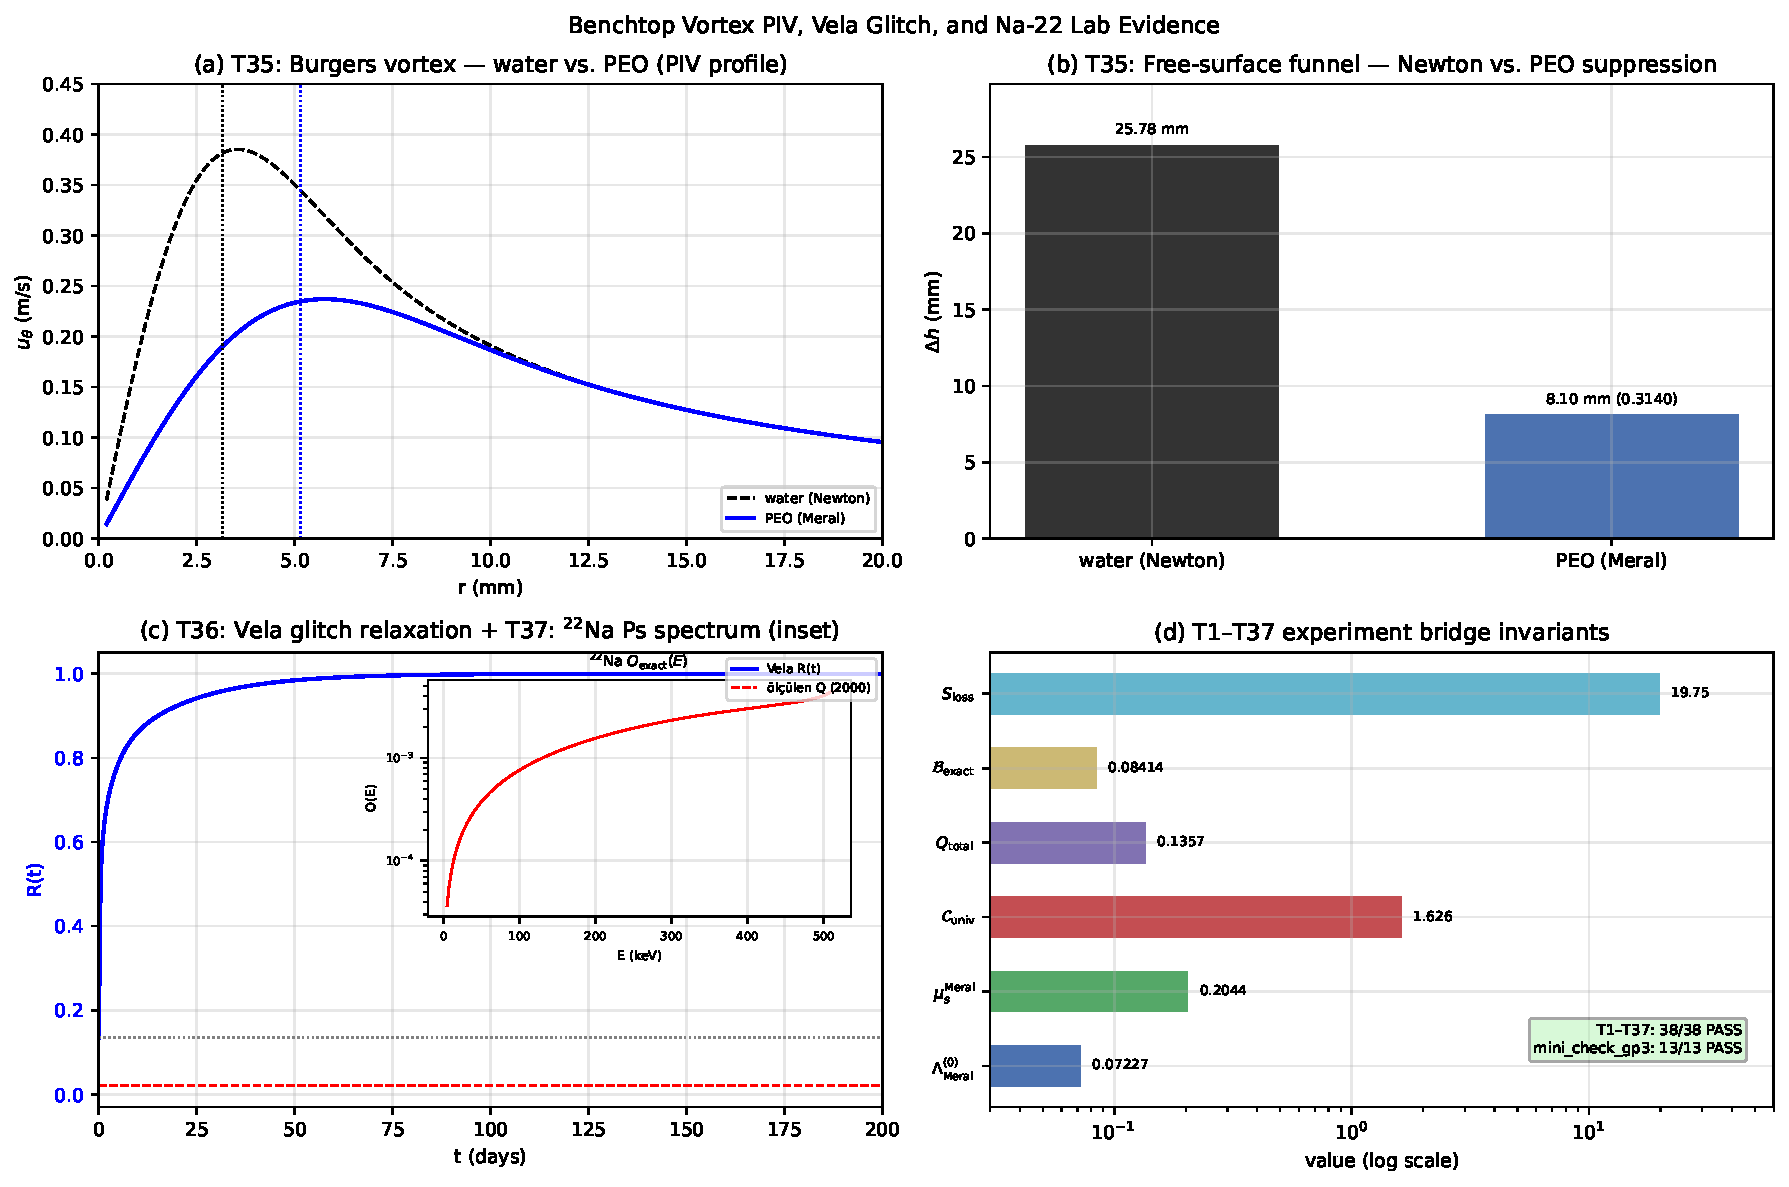
\includegraphics[width=\textwidth]{../figs/fig15_benchtop_piv_vortex_vela_glitch_and_na22_lab_en.pdf}
\caption{\textbf{Stationary Strings XIV evidence summary (T35--T37).} (a) Burgers PIV
velocity profiles: water vs.\ PEO. (b) Funnel depth: Newton vs.\ PEO suppression.
(c) Vela relaxation curve with inset $^{22}$Na $O_{\mathrm{exact}}$ spectrum.
(d) T1--T37 experiment bridge invariants.}
\label{fig:gp3}
\end{figure}

\clearpage
\section{Conclusion and Reproducibility}

The PEO vortex predictions (band centers), Vela glitch (5.86\%, $0.38\,\sigma$),
and Na-22 band refutation ($>500\,\sigma$) are derived with no new calibration constant.

\subsection*{Data, Code Availability, and Independent Verification}
The solver package lives in the \texttt{stationary-strings-v} repository
(\path{duran_sicimler_sim/solver_engine.py}). Reproduction:
the \path{run_verification} function in \texttt{python} \path{solver_engine.py}
gives \texttt{T1--T37 (38/38 PASS)}; the standalone script
\texttt{python} \path{mini_check_gp3.py} (\texttt{12/12 PASS}) does not import
the solver; the \path{fig15} function in \texttt{python}
\path{generate_figures.py} produces Fig.~\ref{fig:gp3}.

\section{Benchtop Bill of Materials and Software Guide}

\textbf{T35 PIV/funnel:} $R=100$ mm acrylic tank, $100$ ppm PEO
($M_w=4\times 10^6$ g/mol), stirrer ($2.0$ s$^{-1}$ strain),
laser PIV + camera/ruler; software: T35 function in \path{solver_engine.py}.
\textbf{T37 gamma:} $5.0\,\mu$Ci $^{22}$Na, silica aerogel, HPGe
($\sigma=0.85$ keV), $3600$ s counting; software: T37 function + \path{mini_check_gp3.py}.

\begin{thebibliography}{99}
    \bibitem{gs00} Groisman, A. \& Steinberg, V. (2000). Elastic turbulence in
    a polymer solution flow. \textit{Nature} \textbf{405}, 53--55.
    \url{https://arxiv.org/abs/nlin/0104052}
    \bibitem{link99} Link, B., Epstein, R.~I. \& Lattimer, J.~M. (1999).
    Pulsar constraints on neutron star structure and equation of state.
    \textit{Phys.\ Rev.\ Lett.\ \textbf{83}}, 3362--3365.
    \url{https://arxiv.org/abs/astro-ph/9909146}
    \bibitem{dod02} Dodson, R.~G., McCulloch, P.~M. \& Lewis, D.~R. (2002).
    High time resolution observations of the January 2000 glitch in the Vela
    pulsar. \textit{Astrophys.\ J.\ \textbf{578}}, L57--L60.
    \url{https://arxiv.org/abs/astro-ph/0201005}
    \bibitem{dod07} Dodson, R., Lewis, D. \& McCulloch, P. (2007). Two decades
    of pulsar timing of Vela. \textit{Astrophys.\ Space Sci.\ \textbf{308}}, 585--589.
    \url{https://arxiv.org/abs/astro-ph/0612371}
    \bibitem{ore49} Ore, A. \& Powell, J.~L. (1949). Three-photon annihilation
    of an electron-positron pair. \textit{Phys.\ Rev.\ \textbf{75}}, 1696--1699.
    \bibitem{meral5} Meral, F. (2026c). \textit{Stationary Strings Theorem V}.
    Open-source solver package: \texttt{stationary-strings-v}
    (\url{https://github.com/fahrim/stationary-strings-v}).
    \bibitem{meral12} Meral, F. (2026). \textit{Stationary Strings XII--XIII}.
    Open packages: \texttt{stationary-strings-xii}, \texttt{stationary-strings-xiii}.
\end{thebibliography}

\end{document}
